\chapter{Research Approach}
\label{chap:research}

In this chapter, we describe the research approach and methodology, grounded
initially in hardware-software co-design and now in
hardware-software-formal co-design, used to develop the CHERI protection model and its ISA instantiations in MIPS, RISC-V, and ARMv8-A.

\section{Motivation}

The CHERI protection model provides a sound and formally based architectural
foundation for the principled development of highly
trustworthy systems.
The CHERI approach builds on and extends decades of research into hardware and
operating-system security.\footnote{Levy's {\em Capability-Based Computer Systems}~\cite{levy:capabilities} provides a
detailed history of segment- and capability-based designs through the early
1990s~\cite{levy:capabilities}.
However, it leaves off just as the transition to microkernel-based capability systems such as
Mach~\cite{accetta:mach}, L4~\cite{liedtke:l4}, and, later, seL4~\cite{klein:sel4}, as
well as capability-influenced virtual machines such as the Java Virtual Machine~\cite{Gong99},
begins.
Chapter~\ref{chap:historical} discuss historical influences on our work in greater detail.}
However, some of the historic approaches that CHERI incorporates (especially capability architectures)
have not been adopted in commodity hardware designs.
In light of these past transition failures, a reasonable question
is ``Why now?''
What has changed that could allow CHERI to succeed where
so many previous efforts have failed?
Several factors have motivated our decision to begin and carry out this project:

\begin{itemize}
\item Dramatic changes in threat models, resulting from ubiquitous
connectivity and pervasive uses of computer technology in many
diverse and widely used applications such as wireless mobile
devices, automobiles, and critical infrastructure.
In addition, cloud computing and storage, robotics, software-defined
networking.  safety of autonomous systems, and the Internet of Things have
significantly widened the range of vulnerabilities that can be exploited.

\item An extended ``arms race'' of inevitable vulnerabilities and novel new
attack mechanisms has led to a cycle of ``patch and pray'': systems will be
found vulnerable, and have little underlying robustness to attackers should
even a single vulnerability be found.
Defenders must race to patch systems as vulnerabilities are announced -- and
vulnerabilities may have long half-lives in the field, especially unpublicized ones.
There is a strong need for underlying architectures that offer stronger
inherent immunity to attacks; when successful attacks occur, robust
architectures should yield fewer rights to attackers, minimize gained attack
surfaces, and increase the work factor for attackers.

\item New opportunities for research into (and possible revisions of)
hardware-software interfaces, brought about by programmable hardware
(especially FPGA soft cores)
and complete open-source software stacks such as
FreeBSD~\cite{mckusick:freebsd} and LLVM~\cite{LA04}.

\item An increasing trend towards exposing inherent hardware parallelism
through virtual machines and explicit software
multi-programming, and an increasing awareness of information flow
for reasons of power and performance that may align well with the
requirements of security.

\item Emerging advances in programming languages, such as the ability
to map language structures into protection parameters to
more easily express and implement various policies.

\item Reaching the tail end of a ``compatibility at all costs'' trend in
CPU design, due to
proximity to physical limits on clock rates and
trends towards heterogeneous and distributed computing.
While ``Wintel'' remains entrenched on desktops, mobile systems -- such as
phones and tablet PCs, as well as appliances and embedded devices -- are
much more diverse, running on a wide variety of instruction set architectures
(especially ARM and MIPS).

\item Similarly,
new diversity in operating systems has arisen, in which commercial
products such as Apple's iOS and Google's Android extend open-source systems
such as FreeBSD, Mach~\cite{accetta:mach}, and Linux.
These new platforms abandon many traditional constraints, requiring
that rewritten
applications conform to new security models, programming languages,
hardware architectures, and user-input modalities.

\item Development of {\em hybrid capability-system models} (notably Capsicum~\cite{Watson10}) that integrate capability-system design tenets into current operating-system and language designs.
With CHERI, we are transposing this design philosophy into the instruction-set architecture.
Hybrid design is a key differentiator from prior capability-system processor designs that have typically required ground-up software-architecture redesign and reimplementation.

\item Significant changes in the combination of hardware, software,
and formal methods to enhance assurance (such as those noted above)
now make possible the development of trustworthy system
architectures that previously were simply too far ahead of their times.
\end{itemize}

\subsection{C-Language Trusted Computing Bases (TCBs)}

Contemporary client-server and cloud computing are based on highly distributed
applications, with end-user components executing in rich execution substrates such
as POSIX applications on UNIX, or AJAX in web browsers.
However, even thin clients are not thin in most practical senses: as with client-server
computer systems, they are built from commodity operating-system kernels, hundreds
of user-space libraries, window servers, language runtime environments, and web
browsers, which themselves include scripting language interpreters, virtual machines,
and rendering engines.
Both server and embedded systems likewise depend on complex (and quite
similar) software stacks.
All require confluence of competing interests, representing multiple sites, tasks, and end users in unified computing environments.

Whereas higher-layer applications are able to run on top of type-safe or constrained
execution environments, such as JavaScript interpreters, lower layers of the system
must provide the link to actual execution on hardware.
As a result, almost all such systems are written in the C programming language;
collectively, this Trusted Computing Base (TCB) consists of many tens of millions of
lines of trusted (but not trustworthy) C and C++ code.
Coarse hardware, OS, and language security models mean that much of this code is
security-sensitive: a single flaw, such as an errant NULL pointer dereference in the kernel,
can expose all rights held by users of a system to an attacker or to malware.

The consequences of compromise are serious, and include loss of data, release of
personal or confidential information, damage to system and data integrity, and even total
subversion of a user's online presence and experience by the attacker (or even
accidentally without any attacker presence!).
These problems are compounded by the observation that the end-user systems are also an
epicenter for multi-party security composition, where a single web browser or office suite
(which manages state, user interface, and code execution for countless different security domains)
must simultaneously provide strong isolation and appropriate sharing.
The results present not only significant risks of compromise that lead to financial loss or
disruption of critical infrastructure, but also frequent occurrences of such events.

Software vulnerabilities appear inevitable;
indeed, an arms race has arisen in new
(often probabilistic) software-based mitigation techniques and exploit
techniques that bypass them.
Even if low-level escalation techniques (such as arbitrary code injection and
code reuse attacks) could be prevented, logical errors and supply-chain
attacks will necessarily persist.
Past research has shown that compartmentalizing applications into components executed
in isolated sandboxes can mitigate exploited vulnerabilities (sometimes referred to as privilege
separation).
Only the rights held by a compromised component are accessible to a successful attacker.
This technique is effectively applied in Google's Chromium web browser, placing HTML
rendering and JavaScript interpretation into sandboxes isolated from the global file system.
Compartmentalization exploits the principle of least privilege: if each software element executes with
only the rights required to perform its task, then attackers lose access to most all-or-nothing
toeholds; vulnerabilities may be significantly or entirely mitigated, and attackers must identify
many more vulnerabilities to accomplish their goals.

\subsection{The Software Compartmentalization Problem}

The {\em compartmentalization problem} arises from attempts to decompose
security-critical software into components running in different security
domains: the practical application of the principle of least privilege to
software.
Historically, compartmentalization of TCB components such as operating system kernels
and central system services has caused significant
difficulty for software developers -- which limits its applicability for large-scale,
real-world applications, and leads to the abandonment of promising research
such as 1990s {\em microkernel} projects.
A recent resurgence of compartmentalization, applied in userspace to system software and applications
such as OpenSSH~\cite{provos:preventingprivesc} and Chromium~\cite{reis:chromium},
and more recently in our own Capsicum project~\cite{Watson10}, has been motivated by a
critical security need; however it has seen success only at very coarse separation granularity due to
the challenges involved.
A more detailed history of work in this area can be found in
Chapter~\ref{chap:historical}.

On current conventional hardware, native applications must be converted to employ message
passing between address spaces (or processes) rather than using a unified address space
for communication, sacrificing programmability and performance by transforming a local
programming problem into a distributed systems problem.
As a result, large-scale compartmentalized programs are difficult to design, write, debug,
maintain, and extend; this raises serious questions about correctness, performance, and most
critically, security.

These problems occur because current hardware provides strong separation
only at coarse granularity via rings and virtual address spaces, making
the isolation of complete applications (or even multiple operating systems)
a simple task, but complicates
efficient and easily expressed separation between tightly coupled software
components.
Three closely related problems arise:

\paragraph{Performance is sacrificed.}
Creating and switching between process-based security domains is expensive due
to reliance on software and hardware address-space infrastructure -- such as a
quickly overflowed Translation Look-aside Buffer (TLB) and large page-table
sizes that can lead to massive performance degradation.
Also, above an extremely low threshold, performance overhead from context
switching between security domains tends to go from simply expensive to
intolerable: each TLB entry is an access-control list, with each object (page)
requiring multiple TLB entries, one for each authorized security domain.

High-end server CPUs typically have TLB entries in the low hundreds, and
even recent network embedded devices reach
the low thousands; the TLB
footprint of fine-grained, compartmentalized software increases with the product of
in-flight security domains and objects due to TLB aliasing, which may easily require
tens or hundreds of thousands of spheres of protection.
The transition to CPU multi-threading has not only failed to relieve this burden,
but actively made it worse: TLBs are implemented using ternary content-addressable
memory (TCAMs) or
other expensive hardware lookup functions, and are often shared between hardware
threads in a single core due to their expense.

Similar scalability critiques apply to page tables, the tree-oriented
in-memory lookup tables used to fill TLB entries.
As physical memory sizes increase, and reliance on independent virtual address
spaces for separation grows, these tables also grow -- competing for cache
and memory space.

In comparison, physically indexed general-purpose CPU caches are several orders
of magnitude larger than TLBs, scaling instead with the working set of code paths
explored or the memory footprint of data actively being used.
If the same data is accessed by multiple security domains, it shares data or code
cache (but not TLB entries) with current CPU designs.

\paragraph{Programmability is sacrificed.}
Within a single address space, programmers
can easily and efficiently share memory between program elements using pointers
from a common namespace.
The move to multiple processes frequently requires the adoption of a distributed
programming model based on explicit message passing, making development,
debugging, and testing more difficult.
RPC systems and higher-level languages are able to mask some (although usually
not all) of these limitations, but are poorly suited for use in TCBs -- RPC systems and
programming language
runtimes are non-trivial, security-critical, and implemented using weaker
lower-level facilities.\footnote{Through extreme
discipline, a programming model can be constructed that maintains synchronized
mappings of multiple address spaces, while granting different rights on memory
between different processes.  This leads to even greater TLB pressure
and expensive context switch operations, as
the layouts of address spaces must be managed using cross-address-space
communication.
Bittau has implemented this model via {\em sthread}s, an OS primitive that
tightly couples UNIX processes via shared memory associated with data types
-- a promising separation approach constrained by the realities of current
CPU design~\cite{bittau:wedge}.}

\paragraph{Security is sacrificed.}
Current hardware is intended to provide robust
shared memory communication only between mutually trusting parties, or at
significant additional expense; granularity of delegation is limited and its
primitives expensive, leading to programmer error and extremely limited use
of granular separation.
Poor programmability contributes directly to poor security properties.

\section{Methodology}

Despite half a century of research into computer systems and software design,
it is clear that security remains a challenging problem -- and an increasingly
critical problem as computer-based technologies find ever expanding deployment
in all aspects of contemporary life, from mobile communications devices to
self-driving cars and medical equipment.
There are many contributing factors to this problem, including the asymmetric
advantage held by attackers over defenders (which cause minor engineering
mistakes to lead to undue vulnerability), the difficulties in assessing -- and
comparing -- the security of systems, and market pressures to deliver products
sooner rather than in a well-engineered state.
Perhaps most influential is the pressure for backward compatibility, required
to allow current software stacks to run undisturbed on new generations of
systems, as well as to move seamlessly across devices (and vendors), locking
in least-common-denominator design choices, and preventing the deployment of
more disruptive improvements that serve security.

Both the current state, and worse, the current direction, support a view that
today's computer architectures (which underlie phenomenal growth of
computer-based systems) are fundamentally ``unfit for purpose'': Rather than
providing a firm foundation on which higher-level technologies can rest, they
undermine attempts to build secure systems that depend on them.
To address this problem, we require designs that mitigate, rather than
emphasize, inevitable bugs, and offer strong and well-understood protections
on which larger-scale systems can be built.
Such technologies can be successful only if transparently adoptable by end
users -- and, ideally, also many software developers.
On the other hand, the resulting improvement must be dramatic to justify
adopting substantive architectural change, and while catering to short-term
problems, must also offer a longer-term architectural vision able to support
further benefit as greater investment is made.

\subsection{Technical Objectives and Implementation}

From a purely technical perspective, the aim of the CHERI project is to
introduce architectural support for the principle of least privilege in order
to encourage its direct utilization at all levels of the software stack.
Current computer architectures make this extremely difficult as they impose
substantial performance, robustness, compatibility, and complexity penalties
in doing so -- strongly disincentivizing adoption of such approaches in
off-the-shelf system designs despite the potential to mitigate broad classes
of known (and also as-yet unknown) vulnerability classes.

Low-level Trusted Computing Bases (TCBs) are typically written in
memory-unsafe languages such as C and C++, which do not offer compatible or
performant protection against pointer corruption, buffer overflows, or other
vulnerabilities arising from that lack of safety not offered directly by the
architecture.
Similarly, software compartmentalization, which mitigates both low-level
vulnerabilities grounded in program representation and high-level application
vulnerabilities grounded in logical bugs, is poorly supported by current MMUs,
leading to substantial (crippling) loss of programmability and performance as
the technique is deployed.

CHERI also seeks to minimize disruption of current designs, in order to
support incremental adoption with significant
transparency: Ideally, CHERI could be ``slid under'' current software stacks
(such as Apple's iOS ecosystem, or Google's Android ecosystem), allowing
non-disruptive introduction, yet providing an immediate reward for adoption.
This requires supporting current low-level languages such as C and C++ more
safely, but also cleanly supplementing MMU-based programming models required
to support current operating systems and virtualization techniques.
These goals have directed many key design choices in the CHERI ISA.

\subsection{Hardware-Software-Formal Co-Design Methodology}

Changes to the hardware-software interface are necessarily disruptive.
The ISA is a ``narrow waist'' abstraction that allows hardware designers to
pursue sophisticated optimization strategies (e.g., to exploit parallelism),
while software developers can simultaneously depend on a (largely unchanging)
interface to build successively larger and more complex artifacts.
Stable ISAs have allowed the development of operating systems and application
suites that can operate successfully on a range of systems, and that outlast
the specific platforms on which they were developed.

This structure is inherently predisposed to non-disruption, as platforms that
incur lower adoption costs will be preferred to those that have higher costs.
However, substantive changes in underlying program representation, such as to
support greater memory safety or fine-grained compartmentalization required to
dramatically improve security, require changes to the ISA.
We therefore aimed to:

\begin{itemize}
\item Iteratively explore disruptions to the ISA, projecting changes both up
  into the software stack including operating systems, compilers, and
  applications (to assess impact on compatibility and security), as well as
  down into microarchitecture (assessing impact on performance and viability).

\item Start with a conventional and well-established 64-bit RISC ISA, rather
  than re-invent the wheel for general-purpose computation, to benefit from
  existing mature software stacks that could then be used for validation.

  For the first few years of the project, we worked with 64-bit MIPS, but we
  have more recently worked with RISC-V and ARMv8-A.
  These latter two ISAs have offered the opportunity to revisit our
  integration with the architecture ``from scratch,'' allowing us to
  substantially refine our approach -- e.g., by employing a merged register
  file.

\item Employ realistic open-source software artifacts, including the FreeBSD
  operating system, Clang/LLVM compiler suite, and an open-source application
  corpus, to ensure that experiments were run with suitable scale, complexity,
  performance footprint, and idiomatic use.

\item Employ realistic hardware artifacts, developing multiple FPGA
  soft-core based processor prototypes able to validate key questions about
  integration with components such as the pipeline and memory hierarchy, as
  well as support performance validation for the full stack including
  software.

  In our 64-bit MIPS work, we utilized a single pipelined processor design.
  For RISC-V, we have employed three microarchitectures spanning a broad
  spectrum: 3-stage and 5-stage pipelined designs, and a superscalar design.

\item Employ formal models of the ISA, to provide an executable gold model for
  testing, from which tests can be automatically generated, and against which
  theorem proving can be deployed to ensure that key properties relied on for
  software security actually hold.

\item Pursue the hypothesis that historic capability-system models, designed
  to support implementation of the principle of least privilege, can be
  hybridized with current software approaches to support compatible and
  efficient fine-grained memory protection and compartmentalization.

\item Take an initially purist capability-system view, incrementally adapting
  that model towards one able to efficiently yet safely support the majority
  of current software use.
  This approach allowed us to retain well-understood monotonicity and
  encapsulation properties, as well as pursue capturing notions of explicit
  valid provenance enforcement and intentional use not well characterized in
  prior capability-system work.
  Appropriately but uncompromisingly represented, these properties have proven
  to align remarkably well with current OS and language designs.

\item Aim specifically to cleanly compose with conventional MMUs and MMU-based
  software designs by providing an in-address-space protection model, as well
  as be able to represent C-language pointers as capabilities.

\item Support incremental adoption, allowing significant benefit to be gained
  through modest efforts (such as re-compiling) for selected software, while
  not disrupting binary-compatible execution of legacy applications.
  Likewise, support incremental deployment of more disruptive
  compartmentalization into key software through greater (but selective)
  investment.

\item Provide primitives that offer immediate short-term benefit (e.g.,
  invulnerability to common pointer-based exploit techniques, scalable
  sandboxing of libraries in key software packages), while also offering a
  longer-term vision for future software structure grounded in strong memory
  safety and fine-grained compartmentalization.
\end{itemize}

\section{Research and Development}
\label{sec:development}

\begin{table}[th]
\begin{center}
\caption{CHERI ISA revisions and major development phases}
\begin{tabular}{llp{3.25in}}
\toprule
  Year(s) & Version & Description \\
\midrule
  2010- & ISAv1 & RISC capability-system model w/64-bit MIPS \\
  2012 & & Capability registers and tagged memory \\
  & & Guarded manipulation of registers \smallskip \\
  2012 & ISAv2 & Extended tagging to capability registers \\
  & & Capability-aware exception handling \\
  & & MMU-based OS with CHERI support \smallskip \\
  2014 & ISAv3~\cite{UCAM-CL-TR-864} & Fat pointers $+$ capabilities, compiler \\
  & & Instructions to optimize hybrid code \\
  & & Sealed capabilities, \insnnoref{CCall}/\insnnoref{CReturn} \smallskip \\
  2015 & ISAv4~\cite{UCAM-CL-TR-876} & MMU-CHERI integration (TLB permissions) \\
  & & ISA support for compressed capabilities \\
  & & Hardware-accelerated domain switching \\
  & & Multicore instructions: \insnnoref{LL}/\insnnoref{SC} variants \smallskip \\
  2016 & ISAv5~\cite{UCAM-CL-TR-891} & CHERI-128 compressed capability model \\
  & & Improved generated code efficiency \\
  & & Initial in-kernel privilege limitations \smallskip \\
  2017 & ISAv6~\cite{UCAM-CL-TR-907} & Mature kernel privilege limitations \\
  & & Further generated code efficiency \\
  & & CHERI-x86 and CHERI-RISC-V sketches \\
  & & Jump-based protection-domain transition \smallskip \\
  2019 & ISAv7~\cite{UCAM-CL-TR-927} & Architecture-neutral protection model \\
  & & A more complete CHERI-RISC-V elaboration \\
  & & Compartment IDs for side-channel resistance \\
  & & 64-bit capabilities for 32-bit architectures \\
  & & Architectural temporal memory safety \\
  & & CHERI Concentrate compressed capabilities \smallskip \\
  2020 & ISAv8~\cite{UCAM-CL-TR-951} & Compressed capabilities in abstract
  model \\
  & & 32- and 64-bit address sizes \\
  & & Deployed sentry capabilities \\
  & & Fully elaborated CHERI-RISC-V \\
  & & MMU-assisted load-side-barrier revocation \\
  & & Richer microarchitectural exploration \\
  & & Synchronized with Arm Morello architecture~\cite{arm-morello} \\
\bottomrule
\end{tabular}

\end{center}
\label{table:cheri-isa-versions}
\end{table}

Between 2010 and 2020, eight major versions of the CHERI model and its
architectural instantiations -- initially MIPS, and later also RISC-V and
ARMv8-A -- developed a
mature hybridization of conventional RISC architecture with a strong (but
software-compatible) capability-system model.
Key research and development milestones can be found in
Figure~\ref{fig:cheri-r-and-d} including major publications.
The major ISA versions, with their development focuses, are described in
Table~\ref{table:cheri-isa-versions}.
This work occurred in several major overlapping phases as aspects of the
approach were proposed, refined, and stabilized through a blend of ISA design,
integrated hardware and software prototyping, and validation of the combined
stack.

\begin{sidewaysfigure}
\begin{center}
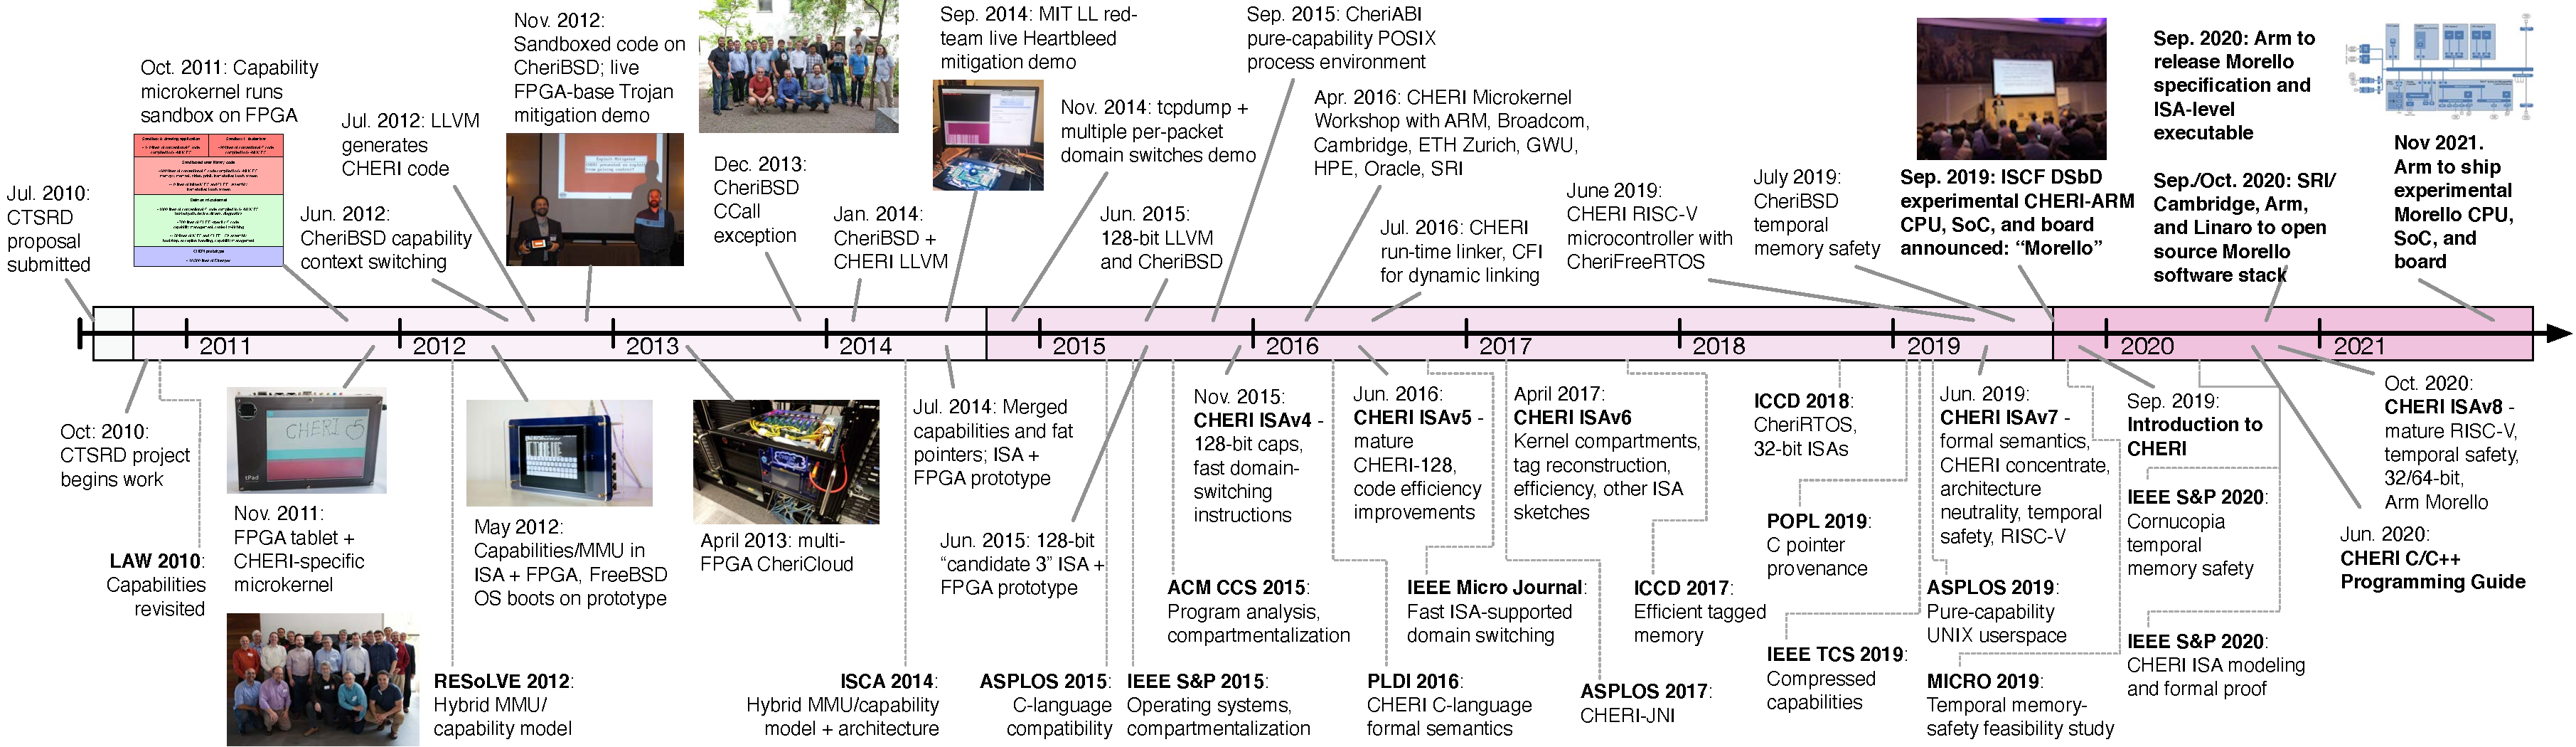
\includegraphics[width=\columnwidth]{20200816-cheri-timeline.pdf}
\caption{CHERI research and development timeline, 2010--2021}
\label{fig:cheri-r-and-d}
\end{center}
\end{sidewaysfigure}

\medskip
\noindent
\textbf{2010--2015: Composing the MMU with a capability-system model}

\nopagebreak
\smallskip
\noindent
A key early design choice was that the capability-system model would be
largely orthogonal to the current MMU-based virtual-memory model, yet also
compose with it cleanly~\cite{woodruff:cheriisca2014}.
We chose to place the capability-system model ``before'' the MMU, causing
capabilities to be interpreted with respect to the virtual, rather than
physical, address space.
This reflected the goal of providing fine-grained memory protection and
compartmentalization within address spaces -- i.e., with respect to the
application-programmer model of memory.

Capabilities therefore protect and implement virtual addresses dereferenced in
much the same way that integer pointers are interpreted in conventional
architectures.
Exceptions allow controlled escape from the capability model by providing
access to privileged capability registers, and execution in privileged rings
grants the ability to manipulate the virtual address space, controlling the
interpretation of virtual addresses embedded in capabilities.

This approach tightly integrates the capability-system model with the pipeline
and register file, requiring that capabilities be first-class primitives
managed by the compiler, held in registers, and so on.
In order to protect capabilities in the virtual address space, we chose to
physically tag them, distinguishing strongly protected pointers from ordinary
data, in turn extending the implementation of physical memory, but also making
that protection entirely independent from (and non-bypassable by) the MMU
mechanism.

\medskip
\noindent
\textbf{2012--2014: Composing C pointers with the capability-system mode}

\smallskip
\noindent
Another key early design choice was the goal of using capabilities to
implement C-language pointers -- initially discretionarily (i.e., as annotated
in the language), and later ubiquitously (i.e., for all virtual addresses in a
more-secure program).
This required an inevitable negotiation between C-language semantics and the
capability-system model, in order to ensure strong compatibility with current
software~\cite{ChisnallCPDP11,Cerberus-PLDI16}.

For example, C embeds a strong notion that pointers point within buffers.
This requires that CHERI capabilities distinguish the notion of current virtual
address from the bounds of the containing buffer -- while also still providing
strong integrity protection to the virtual address.
This led us to compose
fat-pointer~\cite{trevor:cyclone,Nagarakatte:2009:SHC:1542476.1542504,Necula:2002:CTR:503272.503286} and capability
semantics as the capability-system model evolved.

Similarly, we wished to allow all pointers to be represented as capabilities
-- including those embedded within other data structures -- leading naturally
to a choice to mandatorily tag pointers in memory.
A less obvious implication of this approach is that operations such as memory
copying must be capability-oblivious, maintaining the tag across
pointer-propagating memory operations, requiring that data and capabilities
not only be intermingled in memory, but also in register representation.
Capability registers are therefore also tagged, allowing them to hold data or
capabilities, preserving provenance transparently.

As part of this work, we also assisted with the development of new formal
semantics for the C programming language, ensuring that we met the practical
requirements of C programs, but also assisting in formalizing the protection
properties we offer (e.g., strong protection of provenance validity grounded
in an implied pointer provenance model in C).

CHERI should be viewed as providing primitives to support strong C-language
pointer protection, rather than as directly implementing that protection: it
is the responsibility of the compiler (and also operating system and
runtime) to employ capabilities to enforce protections where desired --
whether by specific memory type, based on language annotations, or more
universally.
The compiler can also perform analyses to trade off source-code and binary
compatibility, enforcing protection opportunistically in responding to various
potential policies on tolerance to disruption.

\medskip
\noindent
\textbf{2014--2015: Fine-grained compartmentalization}

\smallskip
\noindent
A key goal of our approach was to differentiate virtualization (requiring
table-based lookups, and already implemented by the MMU) from protection
(now implemented as a constant-time extension to the pointer primitive), which
would avoid table-oriented overheads being imposed on protection.
This applies to C-language protection, but also to the implementation of
higher-level security constructs such as
compartmentalization~\cite{watson15:cheri,watson2016:microjournal}.

Compartmentalization depends on two underlying elements: strong isolation and
controlled communication bridging that isolation.
Underlying monotonicity in capabilities -- i.e., that a delegated reference
to a set of rights cannot be broadened to include additional rights --
directly supports the construction of confined components within address
spaces.
Using this approach, we can place code in execution with only limited
access to virtual memory, constructing ``sandboxes'' (and other more complex
structures) within conventional processes.
The CHERI exception model permits transition to a more privileged component
-- e.g., the operating-system kernel or language runtime -- allowing the
second foundation, controlled communication, to be implemented.

Compartmentalization is facilitated by further extensions to the capability
model, including a notion of ``sealed'' (or encapsulated capabilities).
In CHERI, this is implemented as a software-defined capability: one that has
no hardware interpretation (i.e., cannot be dereferenced), and also strong
encapsulation (i.e., whose fields are immutable).
Other aspects of the model include a type mechanism allowing sealed code and
data capabilities to be inextricably linked; pairs of sealed code
capabilities and data
capabilities can then be used to efficiently describe protection domains via
an object-capability model.
We provide some hardware assistance for protection-domain switching,
providing straightforward parallel implementation of key checks, but leave
the implementation of higher-level aspects of switching to the software
implementation.

Here, as with C-language integration, it is critical that CHERI provide a
general-purpose mechanism rather than enforce a specific policy: the sealed
capability primitive can be used in a broad variety of ways to implement
various compartmentalization models with a range of implied communication
and event models for software.
We have experimented with several such models, including a protection-domain
crossing primitive modeled on a simple (but now strongly protected) function
call, and also on asynchronous message passing.
Our key performance goal was fixed (low) overhead similar to a function call,
avoiding overheads that scale with quantity of memory shared (e.g., as is the
case with table-oriented memory sharing configured using the MMU).

\medskip
\noindent
\textbf{2015--2017: Architectural and microarchitectural efficiency}

\smallskip
\noindent
Side-by-side with development of a mature capability-based architectural
model, we also explored the implications on performance.
This led to iterative refinement of the ISA to improve generated code, but
also substantive efforts to ensure that there was an efficient in-memory
representation of capabilities, as well as microarchitectural implementations
of key instructions.

A key goal was to maintain the principle of a load-store architecture by
avoiding combining computations with memory accesses -- already embodied by
both historic and contemporary RISC architectures.
While pointers are no longer conflated with integer values, a natural
composition of the capability model and ISA maintains that structural goal
without difficulty.

One important effort lay in the reduction from a 256-bit capability (capturing
the requirements of software for 64-bit pointer, 64-bit upper bound, and
64-bit lower bound, as well as additional metadata such as permissions) to a
128-bit compressed representation.
We took substantial inspiration from published work in pointer
compression~\cite{kwon:lowfat}, but found that our C-language compatibility
requirements imposed a quite different underlying model and representation.
For example, it is strictly necessary to support the common C-language idiom
of permitting out-of-bounds pointers (but not dereference), which had been
precluded by many proposed
schemes~\cite{ChisnallCPDP11,Cerberus-PLDI16,davis2019:cheriabi}.
Similarly, the need to support sealed capabilities led to efforts to
characterize the tradeoff between the type space (the number of unique classes
that can be in execution in a CHERI address space) and bounds precision (the
alignment requirements imposed on sealed references).

Another significant effort lay in providing in-memory tags, which are not
directly supported by current DRAM layouts~\cite{joannou2017:tagged-memory, UCAM-CL-TR-936}.
In our initial implementation, we relied on a flat tag table (supported by a
dedicated tag cache).
This imposed a uniform (and quite high) overhead in additional DRAM accesses
across all memory of roughly $10\%$.
We have developed new microarchitectural techniques to improve emulated tag
performance, based on a hierarchical table exploiting sparse use of pointers
in memory, to reduce this overhead to $<2\%$ even with very high pointer
density (e.g., in language runtimes).

\medskip
\noindent
\textbf{2016--2017: Kernel Compartmentalization}

\smallskip
\noindent
Our initial design focus was on supporting fine-grained memory protection
within the user virtual address space, and implicitly, also
compartmentalization.
Beyond an initial microkernel brought up to validate early capability model
variants, kernel prototypes through much of our project have eschewed use of
capability-aware code in the kernel due to limitations of the compiler, but
also because of a focus on large userspace TCBs such as compression libraries,
language runtimes, web browsers, and so on, which are key attack surfaces.

We have more recently returned to in-kernel memory protection and
compartmentalization, where the CHERI model in general carries through without
change -- code executing in the kernel is not fundamentally different from
code executing in userspace.
The key exception is a set of management instructions available to the kernel,
able to manipulate the MMU (and hence the interpretation of capabilities), as
well as control features such as interrupt delivery and exception handling.
We are now extending CHERI to allow the capability mechanism to control access
to these features so that code can be compartmentalized within the kernel.
We are also pursuing changes to the exception-based domain-transition
mechanism used in earlier ISA revisions that shift towards a jump-based model,
which will avoid exception-related overheads in the microarchitecture.

\medskip
\noindent
\textbf{2018--2020: Temporal Memory Safety}

The potential to support strong and deterministic temporal memory safety was
an aim of the CHERI architecture from inception, facilitated by several
architectural features: tagged capabilities allowing accurate identification
of pointers in memory; composition with an MMU to allow invalidation of
portions of the virtual address space; and capability flow control via MMU
and capability permission bits limiting where capabilities could be stored in
memory.
However, we had envisioned this primarily from the perspective of software
compartmentalization, and hence a relatively low overall throughput of
revoked or invalidated capabilities.

With an increased focus on supporting C and C++ memory safety by implementing
all language-level pointers using architectural capabilities, we began to
explore whether heap temporal memory safety could perform adequately using
these techniques.
While for some workloads, they were sufficient, we have expanded the set of
architectural tools to support capability revocation through instructions to
efficiently access tags across regions of memory, and MMU features to allow
tracking of versioned capabilities permitting implementation of load-side
barrier techniques similar to those found in garbage collection appearing in
CHERI ISAv8.
This remains an area of active ongoing research.

\medskip
\noindent
\textbf{2014--2020: Architectural Neutrality}

In our earlier research, CHERI was in all senses an extension to the 64-bit
MIPS ISA.
We took a ``ground up'' view on developing the model, prototyping in a tight
hardware-software co-design loop around the architecture, microarchitecture,
and software, as we brought together ideas about capability-system design and
the baseline ISA.
However, it became apparent that the evolving CHERI protection model in
software related to ideas entirely portable across ISAs: C pointer
implementation, fine-grained memory protection, and software encapsulation.

In 2014, we began a long-running and still ongoing collaboration with Arm
Limited to explore generalizing the model across ISAs, and specifically to
integrate it into the 64-bit ARMv8-A architecture.
This led to the development of a portable architectural model: concept such as
tagged capabilities are essential to CHERI, but not specific to MIPS, ARMv8-A,
or other architectures.
In 2017, in CHERI ISAv6, we sketched integrations of CHERI with the commercial
x86-64 ISA and developing open-source RISC-V ISA.
In CHERI ISAv7, we fully elaborated CHERI-RISC-V, and in CHERI ISAv8 we
polished many aspects of this design based on the experience of implementing a
full hardware-software stack, including three microarchitectures.
In 2019, Arm announced Morello~\cite{arm-morello}, both the integration of
CHERI into ARMv8-A, and also an experimental board implementing the ISA in a
high-end contemporary superscalar processor design.

\section{A Hybrid Capability-System Architecture}

Unlike past research into capability systems, CHERI allows traditional address-space separation, implemented using a memory management unit (MMU), to
coexist with granular decomposition of software within each address space.
Similarly, we have aimed to model CHERI capability behavior not only on strong
capability semantics (e.g., monotonicity), but also to be compatible with
C-language pointer semantics.
As a result, fine-grained memory protection and compartmentalization can be applied selectively throughout existing software
stacks to provide an incremental software migration path.
We envision early deployment of CHERI extensions in selected components of the
TCB's software stack: separation kernels, operating system kernels, programming
language runtimes, sensitive libraries such as those involved in data compression or encryption, and network applications such as web browsers and web
servers.

CHERI addresses current limitations on memory protection and compartmentalization by extending virtual
memory-based separation with hardware-enforced, fine-grained protection within address spaces.
Granular memory protection mitigates a broad range of previously exploitable bugs by coercing common memory-related failures into exceptions that can be handled by the application or operating system, rather than yielding control to the attacker.
The CHERI approach also restores a single address-space programming model for
compartmentalized (sandboxed) software, facilitating efficient, programmable, and robust
separation through the capability model.

We have selected this specific composition of traditional virtual memory with an
in-address-space security model to facilitate technology transition: in CHERI,
existing C-based software can continue to run within processes, and even
integrate with capability-enhanced software within a single process, to provide
improved robustness for selected software components -- and perhaps over time, all
software components.
For example, a sensitive library (perhaps used for image processing) might employ
capability features while executing as part of a CHERI-unaware web browser.
Likewise, a CHERI-enabled application can sandbox and instantiate multiple copies of
unmodified libraries, to efficiently and easily gate access to the rest of application
memory of the host execution environment.

\section{A Long-Term Capability-System Vision}

While we have modeled CHERI as a hybrid capability-system architecture, and in
particular described a well-defined and practical composition with MMU-based
designs, CHERI can also support more ``pure'' capability-oriented hardware and
software designs.
At one extreme in this spectrum, we have begun early experimentation with an
MMU-free processor design offering solely CHERI-based protection for software
use.
We are able to layer a CHERI-specific microkernel over this design, which
executes all programs within a single address-space object-capability model.
This approach might be appropriate to microcontroller-scale systems, to avoid
the cost of an MMU, and in which conventional operating systems might be
inappropriate.
The approach might also be appropriate to very large-scale systems, in which
an MMU is unable to provide granular protection and isolation due to TLB
pressure requiring a shift to very large page sizes.

However, in retaining our primary focus on a hybridization between MMU- and
capability-based approaches, software designs can live at a variety of points
in a spectrum between pure MMU-based and solely CHERI-based models.
A CHERI-based microkernel might be used, for example, within a conventional
operating-system kernel to compartmentalize the kernel -- while retaining an
MMU-based process model.
A CHERI-based microkernel might similarly be used within an MMU-based process
to compartmentalize a large application.
Finally, the CHERI-based microkernel might be used to host solely CHERI-based
software, much as in an MMU-less processor design, leaving the MMU dormant,
or restricted to specific uses such as full-system virtualization -- a task
for which the MMU is particularly well suited.

\section{Threat Model}

%\pgnnote{Model, singular?  Might we have multiple models?  For example,
%    embedded microprocessors might have a different threat model than
%    general-purpose hardware for mobile devices.}
%
%\rwnote{I think I'd take the view that they are the same threat model, as we
%    are concerned with threats originating in locally executing software,
%    whether due to external manipulation (e.g., via network data) or simple
%    local malice.  I'm not sure I perceive a large structural difference for
%    the embedded case -- we are not concerned with physical attacks, etc,
%    where different packaging might affect the story?

CHERI protections constrain code ``in execution'' and allow fine-grained management
of privilege within a framework for controlled separation and communication.
Code in execution can represent the focus of many potentially malicious parties:
subversion of legitimate code in violation of security policies, injection of malicious
code via back doors, Trojan horses, and malware, and also
denial-of-service attacks.
CHERI's fine-grained memory protection mitigates
many common attack techniques by implementing bounds and permission checks,
reducing opportunities for the conflation of code and data, corruption of
control flow, and also catches many common exploitable programmer bugs;
compartmentalization constrains successful attacks via pervasive observance of
the principle of least privilege.

Physical attacks on CHERI-based systems are explicitly excluded from our threat model,
although CHERI CPUs might easily be used in the context of tamper-evident or
tamper-resistant systems.
Similarly, no special steps have been taken in our design to counter undesired
leakage of electromagnetic emanations and certain other side channels such as acoustic inferences:
we take for granted the presence of an
electronic foundation on which CHERI can run.
CHERI will provide a supportive framework for a broad variety of security-sensitive
activities; while not itself a distributed system, CHERI could form a sound foundation for various forms of distributed trustworthiness.

CHERI is an ISA-level protection model that does not address increasingly
important CPU- or bus-level covert and side-channel attacks, relying on the
micro-architecture to limit implicit data flows.
In some sense, CHERI in fact increases exposure: the greater the offers of
protection within a system, the greater the potential impact of unauthorized
communication channels.
As such, we hope side-channel attacks are a topic that we will be able to
explore in future work.
Overall, we believe that our threat model is realistic and will
lead to systems that can be substantially more trustworthy than
today's commodity systems -- while recognizing that ISA-level protections must
be used in concert with other protections suitable to different threat models.

\section{Formal Methodology}

Throughout this project, we apply formal semantics and reasoning techniques to help avoid
system vulnerabilities.
We are (judiciously) applying formal methodology in
five areas:

\begin{enumerate}
\item Early in the project, we developed a formal semantics for the CHERI-MIPS ISA described in
  SRI's Prototype Verification System (PVS) -- an automated theorem-proving
  and model-checking toolchain -- which can be used to verify the
  expressibility of the ISA, but also to prove properties of critical code.
  For example, we are interested in proving the correctness of software-based
  address-space management and domain transitions.
  We are likewise able to automatically generate ISA-level test suites from
  formal descriptions of instructions, which are applied directly to our
  hardware implementation.

\item We developed extensions to the BSV compiler to export
  an HDL description to SRI's PVS and SAL model checker.
  We also developed a new tool (Smten)
for efficient SMT (Satisfiability Modulo Theories) modeling of designs
 (using SRI's Yices), and another tool for
  automated extraction of key properties from larger designs in the
  BSV language, both
  of which greatly simplify formal analysis.
%PS
%   These tools will allow us to verify low-level properties of the hardware design
%   and use the power of model checking and satisfiability solvers to analyze
%   related properties.
% Ideally they will also help link ISA-level specifications with the CPU implementation.


\item We then developed more complete CHERI-MIPS ISA models,
  incorporating both
  MIPS and CHERI instructions, first using the L3 and then the Sail instruction-set description
  languages (both of which support automatic generation of executable
  emulators from formal definitions).
  We have used these as the ``golden model'' of instruction
  behavior, against which our test suite is validated, software implementations can
  be tested in order to generate traces of correct processor execution, and so
  on.
  We have used the L3 and Sail models to identify a number of bugs in multiple hardware
  implementations of CHERI-MIPS, as well as to discover software dependences
  on undefined instruction-set behavior.

\item We have used these L3 and Sail models also as a basis for
  mechanised proof of key architectural security properties.
% PS: this is pasted from new intro text
L3 and Sail support automatic generation of versions of the models in
the definition languages of (variously) the
HOL4, Isabelle, and Coq theorem provers.
Key architectural verification goals including proving not just low-level
properties, such as the monotonicity of each individual instruction
and properties of the CHERI capability compression schemes, but also
higher-level goals such as compartment monotonicity, in which arbitrary code
sequences isolated within a compartment are unable to construct additional
rights beyond those reachable either directly via the register file or
indirectly via loadable capabilities.
We have proven a number of such properties about the CHERI-MIPS ISA, to be
documented in future papers and reports.

% this is now subsumed by the previous bullet
%\item We have proven a number of properties about our ``compressed'' 128-bit
%  capability implementation to ensure that the protection and security
%  properties present in the 256-bit reference semantics (e.g., capability
%  monotonicity) hold of the compressed version -- and that the compression
%  and decompression algorithms are correct.

\item From Sail, we also automatically generate SMT problems, which we
  have used to check properties of our capability compression
  schemes.


\item We have explored how CHERI impacts a formal specification of C-language
  semantics, improving a number of aspects of our C-language compatibility
  (e.g., as relates to conformant handling of the \ccode{intptr_t} type).
\end{enumerate}

\psnote{Taken out the following, as that draft isn't available (as far
  as I can see).  Presumably it described the earlier PVS work -- do
  we need a pointer to something that does describe that?
``A detailed description of formal methods efforts relating to CHERI may
be found in the emerging draft {\em CHERI Formal Methods
Report}~\cite{CHERI-FM15}.''
}

\section{Protection Model and Architecture}

As our work on CHERI has proceeded, we have transitioned from a view in which
CHERI is an ISA extension to 64-bit MIPS to one in which CHERI is a general
protection model that can be expressed through a variety of approaches
and mappings into multiple underlying ISAs.
This report describes a software-facing protection model
(Chapter~\ref{chap:model}) focused on operating systems and compilers,
specific mapping into the 32-bit and 64-bit RISC-V ISA for the purposes of experimentation
and evaluation (Chapters~\ref{chap:architecture}, ~\ref{chap:cheri-riscv}
and~\ref{chap:isaref-riscv}), and architectural sketches for potential integration
into other ISAs (Chapters~\ref{chap:cheri-x86-64} and~\ref{chap:isaref-x86-64} on CHERI-x86-64 and Arm
Morello~\cite{arm-morello}).
However, we have taken a ``ground-up'' approach utilizing hardware-software
co-design to ensure that concrete mapping exist that
satisfies the practical engineering requirements of architecture,
microarchitecture, compiler, operating system, and applications.
At present, our research uses CHERI-RISC-V and Morello.

Our selection of RISC as a foundation for the CHERI capability extensions
is motivated by two factors.
First, simple instruction set architectures are easier to reason about, extend, and implement.
Second, RISC architectures (such as ARM and MIPS) are widely used in network embedded
and mobile device systems such as firewalls, routers, smart phones, and tablets -- markets
with the perceived
flexibility to adopt new CPU facilities, and also an immediate and pressing
need for improved security.
CHERI's new security primitives would also be useful in workstation and server environments,
which face similar security challenges.

CHERI-RISC-V and Arm Morello demonstrate that the abstract CHERI protection
model, as well as our architectural approach, applies to a range of RISC
architectures.
The design principles would also apply to other non-RISC ISAs, such as 32-bit and
64-bit Intel and AMD, but require significantly more adaptation work, as well as careful
consideration of the implications of the diverse set of CPU features found in more CISC-like
architectures.

It is not impossible to imagine pure-software implementations of the CHERI
protection model -- not least, because we use these daily in our work through
both cycle-accurate processor simulations, and a higher-performance but less
microarchitecturally realistic Qemu implementation.
Further, compiler-oriented approaches employing a blend of static checking and
dynamic enforcement could also approximate or implement CHERI protection
semantics (e.g., along the lines of software fault isolation
techniques~\cite{wahbe:sfi} or Google Native Client (NaCl)~\cite{yee:nacl}).
We do, however, hypothesize that these implementations would be difficult to
accomplish without hardware assistance: for example, continuous checking of
program-counter and default data capability bounds, as well as atomic clearing
of tags for in-memory pointers during arbitrary memory writes might come at
substantial expense in software, yet being ``free'' in supporting hardware.

\section{Hardware and Software Prototypes}

As a central part of this research, we have developed reference prototypes of
the CHERI ISA via several CHERI processor designs.
These prototypes allow us to explore,
validate, evaluate, and demonstrate the CHERI approach through realistic
hardware properties and real-world software stacks.
A detailed description of the current prototypes, both from architectural and
practical use perspectives, may be found in our companion papers and technical
reports, described in Section~\ref{sec:publications}.

In our CHERI-MIPS work, we developed two pipelined processor variations that
incorporated our evolving CHERI-MIPS ISA.
These prototypes allowed us to explore ISA design tradeoffs with moderate
microarchitectural realism.
We implement our prototypes in Bluespec SystemVerilog
(BSV)~\cite{Bluespec:TFRG}, allowing us to create highly parameterizable
designs, as well as perform rapid design-space exploration.
Wherever possible, we open source our designs to allow reproduction and reuse
by other researchers.
\jhbnote{Do we want to replace this paragraph with language about
  Piccolo, Flute, and Tooba instead?}

In addition to our BSV implementations, we have also implemented executable
models using first the L3 ISA modeling language~\cite{Fox2015}, and later
SAIL~\cite{sail-popl2019}.
The SAIL descriptions of CHERI-MIPS and CHERI-RISC-V are used for formal
proof, SMT checking, and also directly incorporated into our CHERI ISA
specification.
We also use an adaptation of the QEMU fast ISA accelerator.
\jhbnote{Do we want to drop L3 and MIPS here?}

As the CHERI security model is necessarily a hardware-software model, we have
also performed substantial experimentation with software stacks targeting all
of our ISA instantiations of CHERI.
We have an adaptation of the open-source Clang/LLVM compiler suite, LLD
linker, and GDB debugger, which are able to generate code using CHERI
capabilities.
We have adaptations of the FreeRTOS and FreeBSD operating systems to CHERI,
known as CheriFreeRTOS and CheriBSD.
CheriBSD is portable across all of our CHERI-extended architectures:
CHERI-RISC-V and Morello.
We use CheriFreeRTOS and CheriBSD on our ISA simulations and also on FGPA.

Throughout, we consider metrics such as microarchitectural disruption, Power
Area and Performance (PPA) on FPGA, dynamic benchmark performance, software
language and source-code disruption, and security as part of our evaluation
cycle.
